\chapter{Contexte général}
\section{Introduction générale}
Les émotions sont décrites comme des sentiments intenses dirigés à quelque chose ou quelqu'un en réponse à des événements internes ou externes ayant une signification particulière pour l'individu. Aujourd'hui, l'internet est devenu un moyen clé par lequel les gens expriment leurs émotions, leurs sentiments et leurs opinions. Chaque événement, actualité ou activité dans le monde, est partagé, discuté, publié et commenté sur les réseaux sociaux par des millions de personnes. La capture de ces émotions en texte peut être une source des informations précieuses, qui peuvent être utilisées pour étudier comment les gens réagissent à différentes situations et événements.

Les analystes commerciaux peuvent utiliser ces informations pour suivre les sentiments et les opinions des gens sur leurs produits. Les chefs d’entreprise peuvent analyser la vision globale des personnes réponse à leurs actions ou événements et s'adapter avec cette vision. Ainsi, les analystes de la santé peuvent étudier les sautes d'humeur des individus ou
masses à différents moments de la journée ou en réponse à certains événements. Ces informations peuvent également être utilisé pour formuler l'état mental d'un individu, étudiant son activité sur une période de temps, et éventuellement détecter les risques de dépression.

Le contexte de notre projet est de concevoir et réaliser une application d'analyse des sentiments des tweets en temps réel.

Ce rapport présente l'ensemble d'étapes suivies pour déveloper la solution. Il se divise en 5 chapitres organisés comme suit:
\begin{itemize}
    \item Le premier chapitre "Contexte général" discute l'état de l'art et présente le contexte général du projet.
    \item Le deuxième chapitre "Étude théorique et choix techniques" contient une étude des solutions techniques existantes et discute les différents choix techniques éxplorés dans notre projet.
    \item Le troisième chapitre "Analyse des besoins et spécifications" détermine les différents besoins de notre application et traite son aspect conceptuel.
    \item Le quatrième chapitre "Réalisation" illustre les différentes étapes de la réalisation de l'application.
    \item En conclusions, nous discutons les difficultés rencontrées lors de la réalisation de notre solution et les différents perspectives d'améliorations possibles.
\end{itemize}

\section{Les solutions éxistantes:}
Pour mieux expliquer le contexte général de notre projet, on commence par présenter quelques outils éxistantes au marché:
\begin{itemize}
    \item \bb{Enginuity}: C'est une application Web qui fonctionne différemment de la plupart des outils d'analyse de sentiment libre disponibles. Au lieu d'interroger directement les tweets liés à un certain mot clé, Enginuity permet de rechercher des actualités récentes sur le mot clé.
    Ensuite l'outil interroge Twitter pour calculer le nombre de fois que l'histoire a été partagée. Il analyse également si le sentiment de ces partages est positif ou négatif et donne une note de sentiment globale.
    \item \bb{Steamcrab}: C'est aussi une application Web qui se concentre sur les recherches de mots clés et analyse les tweets selon une échelle bipolaire (positive et négative), comme on peut visualiser ces résultats sur un diagramme de dispersion (scatter plot) ou un diagramme circulaire (pie chart).
    \item \bb{MeaningCloud}: est une API pour l'analyse de texte, y compris l'analyse des sentiments. L'un des avantages de MeaningCloud est que l'API prend en charge un certain nombre d'opérations d'analyse de texte en plus de la classification des sentiments (l'extraction de sujet, la classification grammaticale ou lexicale de texte...).
    \item \bb{NCSU Tweet Sentiment Visualization App} (Application Web): l'un des outils gratuits les plus robustes et hautement fonctionnels pour l'analyse des sentiments sur Twitter. Cette application est facile à utiliser: on doit juste entrer un mot clé et elle extrait automatiquement les tweets récents en nous offrant plusieures options à utiliser (la possibilité de séléctionner des tweets individuels sur le "scatter plot" pour les identifier dans le spectre émotionnel). Ainsi, cette application regroupe automatiquement les tweets en sujets connexes en utilisant des algorithmes d'apprentissage automatique, elle combine alors 'analyse des sentiments avec le regroupement des sujets pour nous aider à comprendre ce que les gens pensent des sujets particuliers.   
\end{itemize}

\section{Présentation générale du projet:}
Notre projet consiste à concevoir et développer une application desktop qui nous permet de rechercher les tweets contenants un mot clé ou une phrase donnés en temps réel, obtenir des statistiques générales sur ces tweets et tracer les changements de leurs sentiments, sauvegarder les graphes tracées ainsi que les tweets et ses analyses sur le disque dur.

\section{Organisation du projet:}
Pour la réalisation de notre projet, on a choisi d'adapter le processus itératif comme méthodologie du travail grâce à la souplesse de cette méthode.

\subsection{Processus itératif:}
Ce processus se décompose en 6 étapes (Figure~\ref{fig:cycleiteratif}).
\begin{figure}
    \centering
    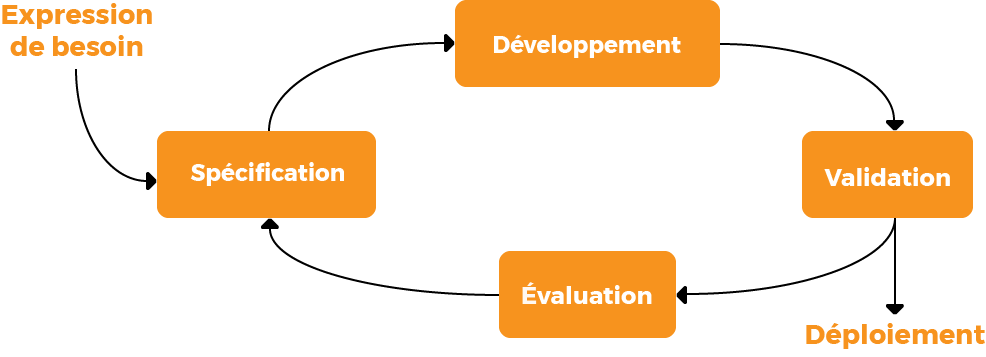
\includegraphics[width=0.8\textwidth]{contexte-generale/assets/cycleiteratif.png}
    \caption{Différentes étapes du cycle itératif}
    \label{fig:cycleiteratif}
\end{figure}

\subsubsection{Expression du besoin:}
La première réunion avec notre encadrant M. Mustapha AMEUR nous a permis de définir les différents besoins: 
\begin{itemize}
    \item Un outil d'analyse des sentiments à partir des tweets où l'utilisateur peut voir un score de positivité et de négativité de chaque tweet, en traçant graphiquement les variations selon le temps.  
\end{itemize}

Ça nous a permis aussi de définir les besoins non fonctionnels concernant notre système:
\begin{itemize}
    \item L’ergonomie : l’application offre une interface conviviale et facile à utiliser.
    \item Le code doit être clair et modulaire pour permettre des futures évolutions ou améliorations. Et d’être paramétrable le plus possible afin d’assurer une simplicité lors changements sans être obliger de modifier le code source.
\end{itemize}

\subsubsection{Spécification:}
Dans cette étape, nous avons choisi les différents outils et technologies qui vont nous aider à satisfaire les besoins définis dans la première étape: 
\begin{itemize}
    \item La conception et le développement d'une application desktop d'analyse des sentiments des tweets en temps réel en Python à l'aide de: Python-twitter, Vader, nltk, TextBlob, PyQt5. Comme on a décidé de former un modèle Naive Bayes basé sur notre propre "dataset". 
\end{itemize} 

\subsubsection{Développement:}
Dans cette étape, nous avons réalisé en concrèt ce qui a été définit en essayant de respecter un exemple d'un ensemble d'étapes de réalisation d'un projet en machine learning (Figure~\ref{fig:machinelearninglifecycle}):
\begin{figure}
    \centering
    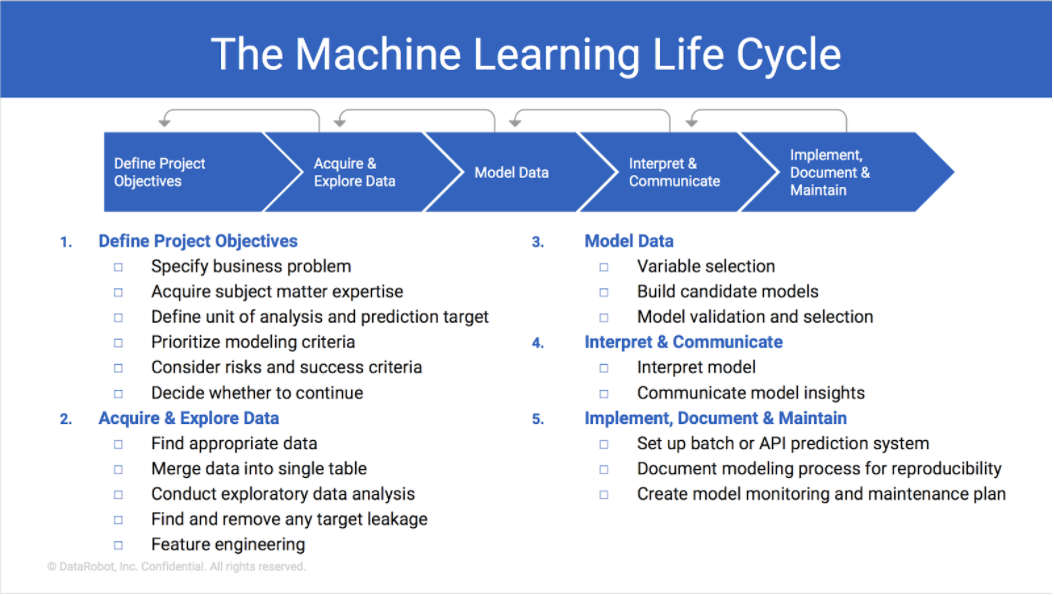
\includegraphics[width=0.9\textwidth]{contexte-generale/assets/machinelearning.png}
    \caption{Exemple d'étapes d'un projet en machine learning}
    \label{fig:machinelearninglifecycle}
\end{figure}

\subsubsection{Validation:}
Ensemble de test permettant d’assurer que le besoin initialement formulé est comblé.

\subsubsection{Évaluation:}
Cette étape nous a permis de faire le point sur les problèmes rencontrés lors des trois précédentes étapes, chose qui nous a aidé à trouver une solution pour accélerer le modèle entrainé (Naive Bayes) après quelques évaluations.

\subsubsection{Déploiement:}
les livrables validés sont déployés et prêts à être utilisé.

\section{Conclusion:}
Dans ce chapitre, nous avons présenter l'idée générale et le contexte de notre projet, comme on a détaillé la méthodologie du travail adaptée lors de la réalisation du projet.
